% Created 2016-03-03 Thu 10:47
\documentclass[11pt]{article}
\usepackage[utf8]{inputenc}
\usepackage[T1]{fontenc}
\usepackage{fixltx2e}
\usepackage{graphicx}
\usepackage{grffile}
\usepackage{longtable}
\usepackage{wrapfig}
\usepackage{rotating}
\usepackage[normalem]{ulem}
\usepackage{amsmath}
\usepackage{textcomp}
\usepackage{amssymb}
\usepackage{capt-of}
\usepackage{hyperref}
\date{\today}
\title{}
\hypersetup{
 pdfauthor={},
 pdftitle={},
 pdfkeywords={},
 pdfsubject={},
 pdfcreator={Emacs 24.5.1 (Org mode 8.3.4)}, 
 pdflang={English}}
\begin{document}

\tableofcontents

\section{Plan to road trip Shenandoah NP \& Blue Ridge Pkwy(and Great Smoky Mountain if possible) this April or May}
\label{sec:orgheadline2}
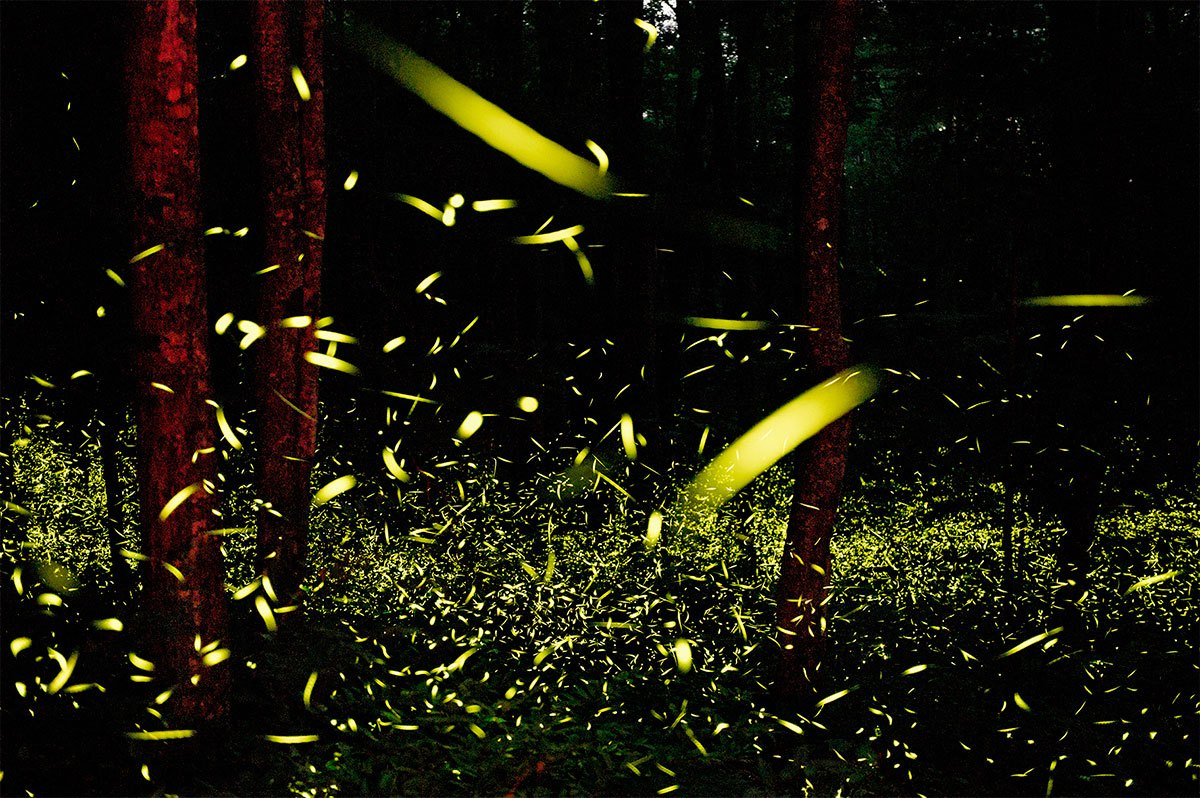
\includegraphics[width=.9\linewidth]{./fireflies-great-smoky-mountains.jpg}

check \href{http://www.heysmokies.com/synchronous-fireflies-in-great-smoky-mountains-june-2016/}{here}

\subsection{{\bfseries\sffamily TODO} important dates}
\label{sec:orgheadline1}
4.10, 4.24, 4.25
\end{document}